%%%%%%%%%%%%%%%%%%%%%%%%%%%%%%%%%%%%%%%%%%%%%%%%
%% Compile: PDFLaTeX BibTeX PDFLaTeX PDFLaTeX
%% Course Slides: Wissenschaftliches Arbeiten
%% Antonio Machicao y Priemer
%%%%%%%%%%%%%%%%%%%%%%%%%%%%%%%%%%%%%%%%%%%%%%%%

\documentclass[a4paper,10pt, bibtotoc]{beamer}
%\documentclass[a4paper,10pt,handout]{beamer}

%%%%%%%%%%%%%%%%%%%%%%%%%
%% PACKAGES & COMMANDS 
%%%%%%%%%%%%%%%%%%%%%%%%%

%%%%%%%%%%%%%%%%%%%%%%%%%%%%%%%%%%%%%%%%%%%%%%%%%%%%
%%%          MyP-Packages   2018.12.08    XeLaTeX
%%%%%%%%%%%%%%%%%%%%%%%%%%%%%%%%%%%%%%%%%%%%%%%%%%%%


%\usepackage[utf8]{inputenc} %XeLaTeX

%% For German texts
\usepackage[ngerman,english]{babel}

%% For English texts
%\usepackage[ngerman,english]{babel}

%% Captions numbered in Beamer 
\setbeamertemplate{caption}[numbered]

%% Change ''Abbildung'' into ''Abb.'' 
%% for: babel
	\renewcommand{\thefigure}{\arabic{figure}}
	\addto\captionsngerman{%
		\renewcommand{\figurename}{Abb.}%
	}
	\renewcommand{\figurename}{Abb.} 

%% Change ''Figure'' into ''Fig.'' 
%% for: babel
	\renewcommand{\thefigure}{\arabic{figure}}
	\addto\captionsenglish{%
		\renewcommand{\figurename}{Fig.}%
	}
%	\renewcommand{\figurename}{Fig.} %% << not needed? 


%% TIPA encoding needs options: T3 & T1
\usepackage[T3,T1]{fontenc}  %not needed in XeLaTeX (?)

%\usepackage{fontspec} % XeLaTeX: Problem: Libertine+Fontspec+TIPA

%% Font
\usepackage{lmodern}
%\usepackage{libertine} % XeLaTeX: Problem: Libertine+Fontspec+TIPA

%% Blind text: \blindtext \Blindtext \blindtext[5] \blindlist{itemize}[x] ...
\usepackage{blindtext}

%% ulem: Strike out
\usepackage[normalem]{ulem}  

%% graphicx: if gb4e is active PDFLaTeX does not accept files with underline. PDFLaTeX accepts files only with .jpg, .png, .pdf endings
\usepackage{graphicx}

%% Math symbols
\usepackage{amsmath}
\usepackage{amsfonts}
\usepackage{amssymb}
\usepackage{MnSymbol} 				% Meaning brackets 

%% Toggles
\usepackage{etoolbox}
	\newtoggle{handout}


%%%%%%%%%%%%%%%%%%%%%%%%%%%%%%%%%%%%%%%%%%%%%%%%%%%%
%%%         Tables & Lists & Columns            
%%%%%%%%%%%%%%%%%%%%%%%%%%%%%%%%%%%%%%%%%%%%%%%%%%%%

% Text in columns: \begin{multicols}{n} \columnbreak \end{multicols}
\usepackage{multicol}
%	\setlength{\columnsep}{.5cm}	

%% Tables with specified width
\usepackage{tabularx}

%% For complex tables
\usepackage{array}

%% For other tables
\usepackage{booktabs}

%% For more than one row in a table
\usepackage{multirow}

%% Special lists: itemize*
\usepackage{mdwlist}


%%%%%%%%%%%%%%%%%%%%%%%%%%%%%%%%%%%%%%%%%%%%%%%%%%%%
%%%          Coloured elements                  
%%%%%%%%%%%%%%%%%%%%%%%%%%%%%%%%%%%%%%%%%%%%%%%%%%%%
%Use xcolor before `gb4e'!
\usepackage{xcolor}


%%%%%%%%%%%%%%%%%%%%%%%%%%%%%%%%%%%%%%%%%%%%%%%%%%%%
%%%          Trees                               
%%%%%%%%%%%%%%%%%%%%%%%%%%%%%%%%%%%%%%%%%%%%%%%%%%%%
%% Forest must be loaded before `gb4e'
\usepackage{forest}
	
	%% Needed for the "actual forest version"
	\useforestlibrary{linguistics}
	\forestapplylibrarydefaults{linguistics}

%% Old forest version
%\usepackage{etex}		%For Forest bug
%\usepackage{../forestold}
	
	
%%%%%%%%%%%%%%%%%%%%%%%%%%%%%%%%%%%%%%%%%%%%%%%%%%%%
%%%          Venndiagram                         
%%%%%%%%%%%%%%%%%%%%%%%%%%%%%%%%%%%%%%%%%%%%%%%%%%%%
%% Package needed: tikz
\usepackage{venndiagram}


%%%%%%%%%%%%%%%%%%%%%%%%%%%%%%%%%%%%%%%%%%%%%%%%%%%%%
%%%%          Verbatim                            
%%%%%%%%%%%%%%%%%%%%%%%%%%%%%%%%%%%%%%%%%%%%%%%%%%%%%
%%`Listings' must be loaded before `gb4', use `verbatim' otherwise
\usepackage{listings}

\lstset{
	language=TeX,
	backgroundcolor=\color{lightgray},
	basicstyle={\footnotesize\ttfamily\color{blue}},
	showstringspaces=false,
	columns=flexible
}
\lstset{literate=%
	{Ö}{{\"O}}1
	{Ä}{{\"A}}1
	{Ü}{{\"U}}1
	{ß}{{\ss}}2
	{ü}{{\"u}}1
	{ä}{{\"a}}1
	{ö}{{\"o}}1
}

%\lstset{%frame=tb,
%	language=Perl,
%	aboveskip=3mm,
%	belowskip=3mm,
%	showstringspaces=false,
%	columns=flexible,
%	basicstyle={\small\ttfamily\color{blue}},
%	numbers=none,
%	%numberstyle=\tiny\color{gray},
%	extendedchars=false,
%	morekeywords={foo},
%	otherkeywords={\#\#},
%	%keywordstyle=\color{blau},
%	%commentstyle=\color{whiteblue},
%	%stringstyle=\color{mauve},
%	breaklines=true,
%	breakatwhitespace=true,
%	tabsize=3
%}


%%%%%%%%%%%%%%%%%%%%%%%%%%%%%%%%%%%%%%%%%%%%%%%%%%%%%
%%%%       Attribute Value Matrices               
%%%%%%%%%%%%%%%%%%%%%%%%%%%%%%%%%%%%%%%%%%%%%%%%%%%%%
\usepackage{../../texfiles-beamer/avm}
%%% Setting of avm (see LSP Guidelines)
	%	\avmfont{\sc}
	%	\avmvalfont{\it}
	\avmfont{\normalfont \scshape} 
	\avmvalfont{\normalfont \itshape} 
%% command to fontify the type values of an avm 
	\newcommand{\tpv}[1]{{\avmjvalfont #1}} 
%% command to fontify the type of an avm and avmspan it
	\newcommand{\tp}[1]{\avmspan{\tpv{#1}}}


%%%%%%%%%%%%%%%%%%%%%%%%%%%%%%%%%%%%%%%%%%%%%%%%%%%%
%%%          IPA                                 
%%%%%%%%%%%%%%%%%%%%%%%%%%%%%%%%%%%%%%%%%%%%%%%%%%%%
%\usepackage[noenc,safe]{tipa}	%in PDFLaTeX
\usepackage[safe]{tipa}	% in XeLaTeX


%%%%%%%%%%%%%%%%%%%%%%%%%%%%%%%%%%%%%%%%%%%%%%%%%%%%
%%%          Vowel diagram                       
%%%%%%%%%%%%%%%%%%%%%%%%%%%%%%%%%%%%%%%%%%%%%%%%%%%%
%\usepackage{vowel}


%%%%%%%%%%%%%%%%%%%%%%%%%%%%%%%%%%%%%%%%%%%%%%%%%%%%
%%%          Bibliography                        
%%%%%%%%%%%%%%%%%%%%%%%%%%%%%%%%%%%%%%%%%%%%%%%%%%%%
\usepackage{natbib}	
	\setcitestyle{notesep={:~}}


%%%%%%%%%%%%%%%%%%%%%%%%%%%%%%%%%%%%%%%%%%%%%%%%%%%%%
%%%%          Settings of the page                
%%%%%%%%%%%%%%%%%%%%%%%%%%%%%%%%%%%%%%%%%%%%%%%%%%%%%

%% (Vertical) Spacing
\usepackage{setspace}
%	\onehalfspacing

%% Space for abbreviations 'i.d.R'
\usepackage{xspace}

%% Margins % >> Option clash for beamer
%\usepackage[a4paper]{geometry} 	
%	\geometry{top=2.5cm, bottom=2.5cm, left=2.5cm, right=2.5cm}


%%%%%%%%%%%%%%%%%%%%%%%%%%%%%%%%%%%%%%%%%%%%%%%%%%%%%
%%%%          Margin notes                        
%%%%%%%%%%%%%%%%%%%%%%%%%%%%%%%%%%%%%%%%%%%%%%%%%%%%%
%% See definition in localcommands.sty, not working with Beamer class
%\usepackage{marginnote}


%%%%%%%%%%%%%%%%%%%%%%%%%%%%%%%%%%%%%%%%%%%%%%%%%%%%%%
%%%%%                Videos                        
%%%%%%%%%%%%%%%%%%%%%%%%%%%%%%%%%%%%%%%%%%%%%%%%%%%%%%
%%Embedding videos >> it does not work
%\usepackage{media9} 


%%%%%%%%%%%%%%%%%%%%%%%%%%%%%%%%%%%%%%%%%%%%%%%%%%%%
%%%          Hyperref & URL                      
%%%%%%%%%%%%%%%%%%%%%%%%%%%%%%%%%%%%%%%%%%%%%%%%%%%%

%\usepackage[hyphens]{url}
\usepackage{url}

%\usepackage{hyperref}

%\usepackage[
%	bookmarksnumbered, % For numbered bookmarks in PDF, not needed for Beamer class
%	hidelinks, %For links without colored borders
%	hyperfootnotes=false %If FNs takes you to the 1st page and not to the FN text
%	]{hyperref}


%%%%%%%%%%%%%%%%%%%%%%%%%%%%%%%%%%%%%%%%%%%%%%%%%%%%
%%%           Examples                           
%%%%%%%%%%%%%%%%%%%%%%%%%%%%%%%%%%%%%%%%%%%%%%%%%%%%

%%% Easy to use: 
%\usepackage{linguex}

%%% gb4e: more powerful than linguex, but with many bugs.
%%% Add gb4e as one of the last packages! 
%\usepackage{gb4e}

%% lsp-gb4eMyP: lsp-Variant of gb4e by MyP
\usepackage{../../texfiles-beamer/lsp-gb4eMyP}

%% (for lsp-gb4eMyP: to add additional information to the right of examples, uncomment the following line)
\usepackage{../../texfiles-beamer/jambox}
%	\jamwidth=2cm\relax 

%% (for lsp-gb4eMyP: if you want the source line of examples to be in italics, uncomment the following line)
% \def\exfont{\it}		


%%%%%%%%%%%%%%%%%%%%%%%%%%%%%%%%%%%%%%%%%%%%%%%%%%%%
%%%           Style Sheet HU                     %%%
%%%%%%%%%%%%%%%%%%%%%%%%%%%%%%%%%%%%%%%%%%%%%%%%%%%%
%% huberlin: Style sheet
\usepackage{../../texfiles-beamer/tex-styleHU/huberlin}

%%% Uni-Tuebingen: Style sheet
%\usepackage{../../texfiles-beamer/tex-styleHU/unituebingen}

%%%%%%%%%%%%%%%%%%%%%%%%%%%%%%%%%%%%%%%%%%%%%%%%%%%%
%%%           MyP-Commands  2018.12.08       
%%%%%%%%%%%%%%%%%%%%%%%%%%%%%%%%%%%%%%%%%%%%%%%%%%%%   


%%%%%%%%%%%%%%%%%%%%%%%%%%%%%%%%
% German quotation marks:
\newcommand{\gqq}[1]{\glqq{}#1\grqq{}}		%double
\newcommand{\gq}[1]{\glq{}#1\grq{}}			%simple


%%%%%%%%%%%%%%%%%%%%%%%%%%%%%%%%
% Abbreviations in German
% package needed: xspace
% Short space in German abbreviations: \,	
\newcommand{\dash}{\mbox{d.\,h.}\xspace}
\newcommand{\idR}{\mbox{i.\,d.\,R.}\xspace}
\newcommand{\su}{\mbox{s.\,u.}\xspace}
\newcommand{\ua}{\mbox{u.\,a.}\xspace}
\newcommand{\va}{\mbox{v.\,a.}\xspace}
\newcommand{\zB}{\mbox{z.\,B.}\xspace}
%\newcommand{\s}{s.~}
%not possibel: \dh --> d.\,h.


%%%%%%%%%%%%%%%%%%%%%%%%%%%%%%%%
%Abbreviations in English
\newcommand{\ao}{a.o.\ }	% among others
\newcommand{\cf}[1]{(cf.~#1)}	% confer = compare
\newcommand{\cfe}[1]{(cf.~(\ref{#1}))}	% compare + example
\newcommand{\ia}{i.a.}	% inter alia = among others
\newcommand{\ie}{i.e.~}	% id est = that is
\newcommand{\fe}{e.g.~}	% exempli gratia = for example
%not possible: \eg --> e.g.~
\newcommand{\vs}{vs.\ }	% versus
\newcommand{\wrt}{w.r.t.\ }	% with respect to


%%%%%%%%%%%%%%%%%%%%%%%%%%%%%%%%
% Dash:
\newcommand{\gs}[1]{--\,#1\,--}


%%%%%%%%%%%%%%%%%%%%%%%%%%%%%%%%
% Rightarrow with and without space
\def\ra{\ensuremath\rightarrow}			%without space
\def\ras{\ensuremath\rightarrow\ }		%with space
\def\la{\ensuremath\leftarrow}
\def\las{\ensuremath\leftarrow\ }


%%%%%%%%%%%%%%%%%%%%%%%%%%%%%%%%
%% X-bar notation

%% Notation with primes (not emphasized): \xprime{X}
\newcommand{\xprime}[1]{#1$^{\prime}$}
\newcommand{\xxprime}[1]{#1$^{\prime\prime}$}
\newcommand{\xxxprime}[1]{#1$^{\prime\prime\prime}$}

%% Notation with primes (emphasized): \exbar{X}
\newcommand{\exprime}[1]{\emph{#1}$^{\prime}$}
\newcommand{\exxprime}[1]{\emph{#1}$^{\prime\prime}$}
\newcommand{\exxxprime}[1]{\emph{#1}$^{\prime\prime\prime}$}

% Notation with zero and max (not emphasized): \xbar{X}
\newcommand{\xzero}[1]{#1$^{0}$}
\newcommand{\maxbar}[1]{#1$^{\textsc{max}}$}

% Notation with zero and max (emphasized): \xbar{X}
\newcommand{\ezerobar}[1]{\emph{#1}$^{0}$}
\newcommand{\emaxbar}[1]{\emph{#1}$^{\textsc{max}}$}

%% Notation with bars (already implemented in gb4e):
% \obar{X}, \ibar{X}, \iibar{X}, \mbar{X} %Problems with \mbar!
% $\overline{}$
%
%% Without gb4e:
\newcommand{\overbar}[1]{\mkern 1.5mu\overline{\mkern-1.5mu#1\mkern-1.5mu}\mkern 1.5mu}
%
%%% OR:
%\newcommand{\ibar}[1]{$\overline{\textrm{#1}}$}
%\newcommand{\iibar}[1]{$\overline{\overline{\textrm{#1}}}$}
%% (emphasized):
\newcommand{\eibar}[1]{$\overline{#1}$}
\newcommand{\eiibar}[1]{\overline{$\overline{#1}}$}


%%%%%%%%%%%%%%%%%%%%%%%%%%%%%%%%
%% Subscript & Superscript: no italics inside math mode
\newcommand{\down}[1]{\textsubscript{#1}}
\newcommand{\downm}[1]{_{\textrm{#1}}}

\newcommand{\up}[1]{\textsuperscript{#1}}
\newcommand{\upm}[1]{^{\textrm{#1}}}


%%%%%%%%%%%%%%%%%%%%%%%%%%%%%%%%
%% Small caps subscripts
\newcommand{\scdown}[1]{\textsubscript{\textsc{#1}}}


%%%%%%%%%%%%%%%%%%%%%%%%%%%%%%%%%
%%% Shorter Underline
%\DeclareTextCommand{\_}{T1}{\leavevmode \kern.06em\vbox{\hrule width.4em}}


%%%%%%%%%%%%%%%%%%%%%%%%%%%%%%%%
%% Object- and Meta-language marking:
%\newcommand{\obj}[1]{\glqq{}#1\grqq{}}		%German double quotes
%\newcommand{\obj}[1]{``#1''}					  %English double quotes
\newcommand{\obj}[1]{\emph{#1}}                 %Emphasising
\newcommand{\term}[1]{\textsc{#1}}              %for abbreviated terminology


%%%%%%%%%%%%%%%%%%%%%%%%%%%%%%%%
% Size:
\newcommand{\size}[1]{{\footnotesize #1}}	% f.e. resize citations


%%%%%%%%%%%%%%%%%%%%%%%%%%%%%%%%
%% for LaTeX terminology: package names, environments, commands
\newcommand{\ltxterm}[1]{{\footnotesize \texttt{#1}}}
\newcommand{\ltxpack}[1]{{\footnotesize \texttt{#1}}}


%%%%%%%%%%%%%%%%%%%%%%%%%%%%%%%%
% Short cuts (<STRG + ALT>):
%\newcommand{\short}[1]{\texttt{\textsc{#1}}}		%Emphasising
\newcommand{\short}[1]{$\langle$\texttt{\textsc{#1}}$\rangle$}		%Emphasising


%%%%%%%%%%%%%%%%%%%%%%%%%%%%%%%%
% Writing text with colour:
% package needed: xcolor
% Command \alert{} in Beamer >> red
\newcommand{\blue}[1]{\textcolor{blue}{#1}}
\newcommand{\green}[1]{\textcolor{green}{#1}}
\newcommand{\red}[1]{\textcolor{red}{#1}}


%%%%%%%%%%%%%%%%%%%%%%%%%%%%%%%%
%% Marking text with colour: 
%%% package needed: color
\newcommand{\clrr}[1]{\colorbox{red}{#1}}
\newcommand{\clry}[1]{\colorbox{yellow}{#1}}


%%%%%%%%%%%%%%%%%%%%%%%%%%%%%%%%
%% Semantic types (<e,t>), features, variables and graphemes in angled brackets 

%%% types and variables, in math mode: angled brackets + italics + no space
%\newcommand{\type}[1]{$<#1>$}

%%% OR more correctly: 
%%% Types and Variables: chevrons! + text in math mode (italics + no space)
\newcommand{\type}[1]{$\langle #1 \rangle$} %% In Math Mode, only single types
\newcommand{\typem}[1]{\langle #1 \rangle } %% Mathmode extra, complex types

%%% Features and Graphemes: chevrons! + normal font
\newcommand{\ab}[1]{$\langle$#1$\rangle$} %% no italics
\newcommand{\abe}[1]{$\langle$\emph{#1}$\rangle$} %% italics


%%%%%%%%%%%%%%%%%%%%%%%%%%%%%%%%
%% Function symbol in Beamer Class!
%% italics and serif
\newcommand{\func}{\emph{\textrm{f}}}
\newcommand{\gunc}{\emph{\textrm{g}}}
\newcommand{\chiF}[1]{\chi _{\textrm{#1}}} 


%%%%%%%%%%%%%%%%%%%%%%%%%%%%%%%%
%% HPSG: Features and Values!
\newcommand{\wert}[1]{\emph{#1}}		%Values & Types
\newcommand{\val}[1]{\emph{#1}}		%Values & Types
\newcommand{\feat}[1]{\textsc{#1}}	%Features


%%%%%%%%%%%%%%%%%%%%%%%%%%%%%%%%
%% (Syntactic) Trees
% package needed: forest
%
%%% Setting for simple trees
%\forestset{
%	sn edges/.style={for tree={parent anchor=south, child anchor=north}}
%}

%%% Setting for complex trees
%\forestset{
%	sn edges/.style={for tree={parent anchor=south, child anchor=north,align=center,base=bottom,where n children=0{tier=word,inner xsep=0pt,outer sep=0pt}{}}}, 
%background tree/.style={for tree={text opacity=0.2,draw opacity=0.2,edge={draw opacity=0.2}}}
%}
%
%\newcommand\HideWd[1]{%
%	\makebox[0pt]{#1}%
%}


%%%%%%%%%%%%%%%%%%%%%%%%%%%%%%%%
%% Outputbox
\newcommand{\outputbox}[1]{\noindent\fbox{\parbox[t][][t]{0.98\linewidth}{#1}}\vspace{0.5em}}


%%%%%%%%%%%%%%%%%%%%%%%%%%%%%%%%
% Margin notes: \myp{NOTE}
% package needed: marginnote
\renewcommand{\marginfont}{\singlespacing}
\renewcommand{\marginfont}{\footnotesize}
\renewcommand{\marginfont}{\color{black}}

\newcommand{\myp}[1]{%
	\marginnote{%
		\begin{spacing}{1}
			\vspace{-\baselineskip}%
			\color{red}\scriptsize#1
		\end{spacing}
	}
}


%%%%%%%%%%%%%%%%%%%%%%%%%%%%%%%%
%% Corpora & Grammmars
\newcommand{\DWDS}[1]{DWDS\nocite{DWDS}: #1}
 
\newcommand{\CREA}{\citetext{CREA \citeyear{CREA}}}
\newcommand{\CREAA}{\citetext{CREA \citeyear{CREAA}}}
\newcommand{\CORPES}{\citetext{CORPES \citeyear{CORPES}}}

\newcommand{\DECOW}{\citetext{DECOW \citeyear{SchaeferR15a}}}
\newcommand{\ESCOW}{\citetext{ESCOW \citeyear{SchaeferR&Co12a}}}

\newcommand{\RAEa}[1]{RAE, \citeyear[#1]{RAE10a}}
\newcommand{\RAEb}[1]{RAE, \citeyear[#1]{RAE10b}}


%%%%%%%%%%%%%%%%%%%%%%%%%%%%%%%%
%% Literature and Appendix
\newcommand{\backupbegin}{
	\newcounter{finalframe}
	\setcounter{finalframe}{\value{framenumber}}
}
\newcommand{\backupend}{
	\setcounter{framenumber}{\value{finalframe}}
}


%%%%%%%%%%%%%%%%%%%%%%%%%%%%%%%%%%%%%%%%%%%%%%%%%%%%
%%%          Useful commands                    
%%%%%%%%%%%%%%%%%%%%%%%%%%%%%%%%%%%%%%%%%%%%%%%%%%%%


%%%%%%%%%%%%%%%%%%%%%%%%%%%%%%%%%%%
%%%%%%%%%%%%%%%%%%%%%%%%%%%%%%%%%%%
%\section{XY}
%%\frame{
%%\begin{multicols}{2}
%%\frametitle{~}
%%	\tableofcontents[currentsection]
%%\end{multicols}
%%}
%%%%%%%%%%%%%%%%%%%%%%%%%%%%%%%%%%%
%
%\begin{frame}{XY}
%
%\begin{itemize}
%	\item XY
%\end{itemize}
%
%\end{frame}


%%%%%%%%%%%%%%%%%%%%%%%%%%%%%%%%%%%
%%%%%%%%%%%%%%%%%%%%%%%%%%%%%%%%%%%
%\iftoggle{handout}{
%	
%%%%%%%%%%%%%%%%%%%%%%%%%%%%%%%%%%%
%\begin{frame}
%%\frametitle{Bücher \& Artikel}
%	
%Test Toggle ON
%	
%\end{frame}
%
%}
%%% END handout true 
%%% BEGIN handout false
%{
%%%%%%%%%%%%%%%%%%%%%%%%%%%%%%%%%%%
%
%%% EMPTY
%
%}%% END HO-Toggle
%%%%%%%%%%%%%%%%%%%%%%%%%%%%%%%%%%%


%%%%%%%%%%%%%%%%%%%%%
%% COMMENTING BLOCKS
% \if0    \fi 

%%%%%%%%%%%%%%%%%%%%%
%% FOR ITEMS:
%\begin{itemize}
%  \item<2-> from point 2
%  \item<3-> from point 3 
%  \item<4-> from point 4 
%\end{itemize}
%
% or: \onslide<2->
% or: \visible<overlay specification>{text}
% or: \only<overlay specification>{text}
% or: \pause

%%%%%%%%%%%%%%%%%%%%%
%% JAMBOX FOR EXAMPLES:
%\ea 
%\settowidth\jamwidth{ Test} 
%Die Studierenden, die weitgehend von Stipendien leben, erhalten einen Mietzuschuss. 
%\jambox{Test}
%\z 

%%%%%%%%%%%%%%%%%%%%%
%% VERTICAL SPACE:
% \vspace{.5cm}
% \vfill

%%%%%%%%%%%%%%%%%%%%%
% RED MARKING OF TEXT:
%\alert{bis spätestens Mittwoch, 18 Uhr}

%%%%%%%%%%%%%%%%%%%%%
%% RESCALE BIG TABLES:
%\scalebox{0.8}{
%For Big Tables
%}

%%%%%%%%%%%%%%%%%%%%%
%% BLOCKS:
%\begin{alertblock}{Title}
%Text
%\end{alertblock}
%
%\begin{block}{Title}
%Text
%\end{block}
%
%\begin{exampleblock}{Title}
%Text
%\end{exampleblock}

%%%%%%%%%%%%%%%%%%%%%
%% MINIPAGE:
%\begin{minipage}[ÄUSSERE POSITION][HÖHE][INNERE POSITION]{BREITE}
%	Beispieltext
%\end{minipage}
%
%% MINIPAGE EXAMPLE:
%\begin{minipage}[b][][c]{.45\textwidth}
%	\onslide<2->
%	\begin{figure}
%		\centering
%		\includegraphics[scale=.1]{../material/Vierecke-Fee1}
%		\caption{Vierecke 1}
%	\end{figure}
%\end{minipage}
%%
%\begin{minipage}[b][][c]{.45\textwidth}
%	\onslide<3->
%	\begin{figure}
%		\centering
%			\includegraphics[scale=.1]{../material/Vierecke-Fee2}
%		\caption{Vierecke 2}
%	\end{figure}
%\end{minipage}	
%%

%%%%%%%%%%%%%%%%%%%%%
%% VIDEO:
%\begin{frame}
%\frametitle{Vor fast 54 Jahren in Berlin \dots}
%
%\begin{center}
%	\includemedia[
%	width=0.9\linewidth,height=0.506\linewidth,
%	activate=pageopen,
%	flashvars={
%		modestbranding=1 % no YT logo in control bar
%		&autohide=1 % controlbar autohide
%		&showinfo=0 % no title and other info before start
%		&rel=0 % no related videos after end
%		&playsinline=0
%		&start=28.5
%	}
%	]{}{http://www.youtube.com/v/NaZ3onbUrew}
%\end{center}
%
%\end{frame}


%%%%%%%%%%%%%%%%%%%%%%%%%%%%%%%%%%%%%%%%%%%%%%%%%%%%
%%%          NOTES: To Check                    
%%%%%%%%%%%%%%%%%%%%%%%%%%%%%%%%%%%%%%%%%%%%%%%%%%%% 

% Do I use ``'' or \emph{•} for object language?



%%%%%%%%%%%%%%%%%%%%%%%%%%%%%%%%%%%%%%%%%%%%%%%%%%%%
%%%             Preamble's End                   
%%%%%%%%%%%%%%%%%%%%%%%%%%%%%%%%%%%%%%%%%%%%%%%%%%%% 

\begin{document}
	
	\togglefalse{handout}
	%\toggletrue{handout}

%%%%%%%%%%%%%%%%%%%%%%%%%%%%%%%%%%%%%%%%%%%%%%%%
%% Compile the master file!
%% 		Slides: Antonio Machicao y Priemer
%% 		Course: Wissenschaftliches Arbeiten
%%%%%%%%%%%%%%%%%%%%%%%%%%%%%%%%%%%%%%%%%%%%%%%%


%%%%%%%%%%%%%%%%%%%%%%%%%%%%%%%%%%%%%%%%%%%%%%%%%%%%
%%%             Metadata                         
%%%%%%%%%%%%%%%%%%%%%%%%%%%%%%%%%%%%%%%%%%%%%%%%%%%%    

\title{
	Wissenschaftliches Arbeiten in der Linguistik\\
	(Technische Übung)
}

\subtitle{\LaTeX\ -- Teil 5: Pakete für Linguisten II}

\author[aMyP]{
	{\small Antonio Machicao y Priemer}
	\\
	{\footnotesize \url{www.linguistik.hu-berlin.de/staff/amyp}}
	%	\\
	%	{\footnotesize \href{mailto:mapriema@hu-berlin.de}{mapriema@hu-berlin.de}}
}

\institute{Institut für deutsche Sprache und Linguistik}

\date{ }

%\publishers{\textbf{6. linguistischer Methodenworkshop \\ Humboldt-Universität zu Berlin}}

%\hyphenation{nobreak}


%%%%%%%%%%%%%%%%%%%%%%%%%%%%%%%%%%%%%%%%%%%%%%%%%%%%
%%%             Preamble's End                   
%%%%%%%%%%%%%%%%%%%%%%%%%%%%%%%%%%%%%%%%%%%%%%%%%%%%      


%%%%%%%%%%%%%%%%%%%%%%%%%%%%%%%%%%%
%%%%%%%%%%%%%%%%%%%%%%%%%%%%%%%%%%%    
%% Title slide 
\begin{frame}
  \HUtitle
\end{frame}


%% Contents slide
\frame{
\begin{multicols}{2}
	\frametitle{Inhaltsverzeichnis}
%	\tableofcontents[hideallsubsections]
	\tableofcontents
	%[pausesections]
\end{multicols}
	}


%%%%%%%%%%%%%%%%%%%%%%%%%%%%%%%%%%%%
%%%%%%%%%%%%%%%%%%%%%%%%%%%%%%%%%%%%
%% Extra literature

\nocite{Freitag&MyP15a}
\nocite{Knuth1986}
\nocite{Kopka94a}
\nocite{MyP17c}
\nocite{MyP&Kerkhof16a}
	
%%%%%%%%%%%%%%%%%%%%%%%%%%%%%%%%%%%%
%%%%%%%%%%%%%%%%%%%%%%%%%%%%%%%%%%%%


%%%%%%%%%%%%%%%%%%%%%%%%%%%%%%%%%%%%
%%%%%%%%%%%%%%%%%%%%%%%%%%%%%%%%%%%%
%%% Basic literature for these slides

\begin{frame}
\frametitle{Grundlage \& empfohlene Lektüre}

\dots basierend auf \citet{Freitag&MyP15a} und auf \citet{MyP&Kerkhof16a}\\
\ras \href{https://www.researchgate.net/publication/279514740_LATEX-Einfuhrung_fur_Linguisten}{LINK}

\end{frame}


%%%%%%%%%%%%%%%%%%%%%%%%%%%%%%%%%%
%%%%%%%%%%%%%%%%%%%%%%%%%%%%%%%%%%
\section{Strukturbäume}
\frame{
	\frametitle{~}
	\begin{multicols}{2}
		\tableofcontents[currentsection,hideallsubsections]
	\end{multicols}
}
%%%%%%%%%%%%%%%%%%%%%%%%%%%%%%%%%%
%%%%%%%%%%%%%%%%%%%%%%%%%%%%%%%%%%

\begin{frame}[fragile]
\frametitle{Strukturbäume}

Es gibt verschiedene Pakete für um Strukturbäume zu zeichnen:

\begin{itemize}
	\item \ltxpack{qtree}
	\item \ltxpack{pstrees} (anspruchsvollere Syntax, aber mächtiger als \ltxpack{qtree})
	\item \ltxpack{tikz-qtree}
	\item \alert{\ltxpack{forest}} (einfache Syntax, mächtiger als \ltxpack{pstrees} und \ltxpack{qtree})
	\item \dots 
\end{itemize}

Wir werden hier mit \ltxpack{forest} arbeiten, für eine kurze Beschreibung der anderen Pakete siehe \citet{Freitag&MyP15a} oder \citet{Linke05a}.
\end{frame}


%%%%%%%%%%%%%%%%%%%%%%%%%%%%%%%%%%
%%%%%%%%%%%%%%%%%%%%%%%%%%%%%%%%%%
\subsection{forest laden}
%\frame{
%	\frametitle{~}
%	\begin{multicols}{2}
%		\tableofcontents[currentsection,hideallsubsections]
%	\end{multicols}
%}
%%%%%%%%%%%%%%%%%%%%%%%%%%%%%%%%%%
%%%%%%%%%%%%%%%%%%%%%%%%%%%%%%%%%%

\begin{frame}[fragile]
\frametitle{forest laden}

Laden Sie das Paket:

\begin{lstlisting}
\usepackage{forest}
\end{lstlisting}

\begin{itemize}
	\item \ltxpack{forest} bietet eine Reihe von Features für linguistische Strukturbäume. Man kann diese Features als Paket-Option laden (oder mit einem Extrabefehl, der die Linguistik-Bibliothek lädt).
\end{itemize}	

\begin{lstlisting}
\usepackage[linguistics]{forest}
\end{lstlisting}

\end{frame}


%%%%%%%%%%%%%%%%%%%%%%%%%%%%%%%%%%
\begin{frame}[fragile]
%\frametitle{Baumstrukturen}

\begin{minipage}[b]{.48\textwidth}
\begin{figure}
	\centering
	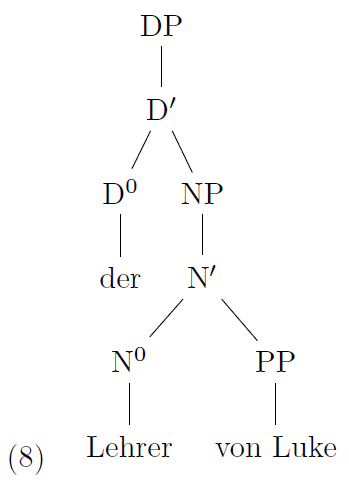
\includegraphics[width=.6\linewidth]{../../texfiles-beamer/tex-material/WissArb-latex/forest2}	
	\caption{ohne Option}
\end{figure}
\end{minipage}
%%
%%
\begin{minipage}[b]{.48\textwidth}
	\begin{figure}
		\centering
		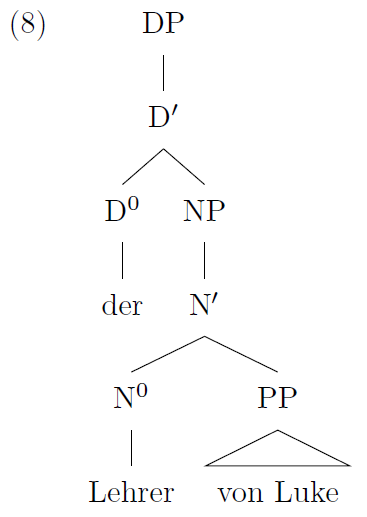
\includegraphics[width=.63\linewidth]{../../texfiles-beamer/tex-material/WissArb-latex/forest1}
		\caption{mit Option}	
	\end{figure}
\end{minipage}


\end{frame}


%%%%%%%%%%%%%%%%%%%%%%%%%%%%%%%%%%
\begin{frame}[fragile]
%\frametitle{Baumstrukturen}

\begin{itemize}
	\item Wie bereits erwähnt, definiert \ltxpack{gb4e} bestimmte \LaTeX -Befehle um, die auch für \ltxpack{forest} benötigt werden. Es ist sehr wichtig, dass Sie \alert{zuerst  \ltxpack{forest}} und \alert{erst dann \ltxpack{gb4e}} laden (\ltxpack{gb4e} sollte eines der letzten Pakete sein!)
\end{itemize}


\begin{lstlisting}
\usepackage[linguistics]{forest}

\usepackage{gb4e}
\end{lstlisting}

\end{frame}


%%%%%%%%%%%%%%%%%%%%%%%%%%%%%%%%%%
%%%%%%%%%%%%%%%%%%%%%%%%%%%%%%%%%%
\subsection{forest-Syntax}
%\frame{
%	\frametitle{~}
%	\begin{multicols}{2}
%		\tableofcontents[currentsection,hideallsubsections]
%	\end{multicols}
%}
%%%%%%%%%%%%%%%%%%%%%%%%%%%%%%%%%%
%%%%%%%%%%%%%%%%%%%%%%%%%%%%%%%%%%

\begin{frame}[fragile]
\frametitle{forest-Syntax}

\begin{itemize}
	\item Um Strukturbäume zu zeichnen verwenden Sie die \ltxpack{forest}-Umgebung.
	
	\item Die weitere \ltxpack{forest}-Syntax ist wie die bereits bekannte Klammernotation bei Strukturbäumen.
\end{itemize}


\begin{lstlisting}
\begin{forest}
	[S [NP] [VP]]
\end{forest}
\end{lstlisting}

\ea \begin{forest}
	[S [NP] [VP]]
\end{forest}
\z 

\begin{itemize}
	\item Die Klammernotation können Sie hier üben:
	\url{http://ironcreek.net/phpsyntaxtree/}

\end{itemize}

\end{frame}


%%%%%%%%%%%%%%%%%%%%%%%%%%%%%%%%%%
\begin{frame}[fragile]
%\frametitle{Baumstrukturen}

Bei größeren Bäumen ist es empfehlenswert die Klammernotation \textbf{nicht linear} zu verwenden. Lassen Sie aber \textbf{keine Leerzeilen} in Ihrem Baum, andernfalls bekommen Sie Fehlermeldungen.


\begin{minipage}[t]{.48\textwidth}
\small	
\begin{lstlisting}
\begin{forest}
  [S 
    [NP] 
    [VP
      [NP]
      [V$^{0}$]
    ]
  ]
\end{forest}
\end{lstlisting}

\vs

\begin{lstlisting}
\begin{forest}
[S [NP] [VP [NP] [V$^{0}$]]]
\end{forest}
\end{lstlisting}
\end{minipage}
%%
%%
\begin{minipage}[t]{.48\textwidth}
\begin{figure}

\centering
\begin{forest}
	[S 
	[NP] 
	[VP
	[NP]
	[V$^{0}$]
	]
	]
\end{forest}

\end{figure}

\end{minipage}

\end{frame}


%%%%%%%%%%%%%%%%%%%%%%%%%%%%%%%%%%
%%%%%%%%%%%%%%%%%%%%%%%%%%%%%%%%%%
\subsection{Bäume in Bsp.-Umgebungen}
%\frame{
%	\frametitle{~}
%	\begin{multicols}{2}
%		\tableofcontents[currentsection,hideallsubsections]
%	\end{multicols}
%}
%%%%%%%%%%%%%%%%%%%%%%%%%%%%%%%%%%
%%%%%%%%%%%%%%%%%%%%%%%%%%%%%%%%%%

\begin{frame}[fragile]
\frametitle{Bäume in Bsp.-Umgebungen}


Bei Verwendung der Option \ltxterm{linguistics} können Sie Ihre Bäume \textbf{in Beispielumgebungen einbetten}.


\begin{lstlisting}
\begin{exe}
\ex 
  \begin{forest}
    [S [NP] [VP]]
  \end{forest}
\end{exe}
\end{lstlisting}

\begin{exe}
	\ex 
	\begin{forest}
		[S [NP] [VP]]
	\end{forest}
\end{exe}

\end{frame}


%%%%%%%%%%%%%%%%%%%%%%%%%%%%%%%%%%
%%%%%%%%%%%%%%%%%%%%%%%%%%%%%%%%%%
\subsection{Abkürzungen in Bäumen}
%\frame{
%	\frametitle{~}
%	\begin{multicols}{2}
%		\tableofcontents[currentsection,hideallsubsections]
%	\end{multicols}
%}
%%%%%%%%%%%%%%%%%%%%%%%%%%%%%%%%%%
%%%%%%%%%%%%%%%%%%%%%%%%%%%%%%%%%%

\begin{frame}[fragile]
\frametitle{Abkürzungen in Bäumen}


Mit dem Befehl \lstinline|roof| können Sie \textbf{Knoten abkürzen}.


\begin{lstlisting}
\begin{exe}
\ex 
  \begin{forest}
    [S [NP [Peter, roof]] [VP [schläft sehr lange, roof]]]
  \end{forest}
\end{exe}
\end{lstlisting}

\begin{exe}
	\ex 
	\begin{forest}
		[S [NP [Peter, roof]] [VP [schläft sehr lange, roof]]]
	\end{forest}
\end{exe}

\end{frame}


%%%%%%%%%%%%%%%%%%%%%%%%%%%%%%%%%%
%%%%%%%%%%%%%%%%%%%%%%%%%%%%%%%%%%
\subsection{Glossen oder Übersetzungen}
%\frame{
%	\frametitle{~}
%	\begin{multicols}{2}
%		\tableofcontents[currentsection,hideallsubsections]
%	\end{multicols}
%}
%%%%%%%%%%%%%%%%%%%%%%%%%%%%%%%%%%
%%%%%%%%%%%%%%%%%%%%%%%%%%%%%%%%%%

\begin{frame}[fragile]
\frametitle{Glossen oder Übersetzungen}


Mit \lstinline|\\| können Sie im Baum \textbf{Glossen/Übersetzungen} angeben.


\begin{minipage}[t]{.48\textwidth}
	\small	
\begin{lstlisting}
\begin{forest}
[S 
  [NP 
    [Peter \\ 
    Peter \\ 
    Pedro, roof]
  ] 
  [VP 
    [schläft viel \\ 
    sleeps a lot \\ 
    duerme mucho, roof]
  ]
]
\end{forest}
\end{lstlisting}
\end{minipage}
%%
%%
\begin{minipage}[t]{.48\textwidth}
	
\begin{exe}
	\ex 
	\begin{forest}
		[S [NP [Peter \\ Peter \\ Pedro, roof]] 
		[VP [schläft viel \\ 
		sleeps a lot \\ 
		duerme mucho, roof]]]
	\end{forest}
\end{exe}
\end{minipage}

\end{frame}


%%%%%%%%%%%%%%%%%%%%%%%%%%%%%%%%%%
%%%%%%%%%%%%%%%%%%%%%%%%%%%%%%%%%%
\subsection{Hoch- und tiefgestellt}
%\frame{
%	\frametitle{~}
%	\begin{multicols}{2}
%		\tableofcontents[currentsection,hideallsubsections]
%	\end{multicols}
%}
%%%%%%%%%%%%%%%%%%%%%%%%%%%%%%%%%%
%%%%%%%%%%%%%%%%%%%%%%%%%%%%%%%%%%

\begin{frame}[fragile]
\frametitle{Hoch- und tiefgestellt}

\begin{itemize}
	\item Die Zeichen \lstinline|^| und \lstinline|_| werden für hoch- und tiefgestellte Elemente verwendet. 
	
	\item Diese Zeichen können aber \textbf{nur im Mathematikmodus} benutzt werden \lstinline|$^1$| \lstinline|$_1$|
\end{itemize}
\end{frame}


%%%%%%%%%%%%%%%%%%%%%%%%%%%%%%%%%%
\begin{frame}[fragile]
%\frametitle{Hoch- und tiefgestellt}

\begin{itemize}	
	\item Der \textbf{Default-Skopus} von \lstinline|^| und \lstinline|_| ist nur ein Zeichen, siehe (\ref{ex:BspHochTief}).
	
	\item Um den Skopus zu erweitern, müssen die \textbf{geschwungenen Klammern} \lstinline|{ }| benutzt werden, siehe (\ref{ex:BspKlammer}). 
\end{itemize}

%\begin{minipage}[t]{.52\textwidth}
{\scriptsize
\begin{lstlisting}
\ea \label{ex:BspHochTief}
  \ea X$^Agens$ Y$^Agens oder Patiens$
  \ex X$_Agens$ Y$_Agens oder Patiens$
  \z 
\ex \label{ex:BspKlammer}
  \ea X$^{Agens}$ Y$^{Agens oder Patiens}$
  \ex X$_{Agens}$ 
  Y$_{Agens oder Patiens}$
  \z 
\z 
\end{lstlisting}
}
%\end{minipage}
%%%
%%%
%\begin{minipage}[t]{.47\textwidth}
\ea \label{ex:BspHochTief}
\ea X$^Agens$ Y$^Agens oder Patiens$
\ex X$_Agens$ Y$_Agens oder Patiens$
\z 

\ex \label{ex:BspKlammer}
\ea X$^{Agens}$ Y$^{Agens oder Patiens}$
\ex X$_{Agens}$ Y$_{Agens oder Patiens}$
\z 
\z 
%\end{minipage}

\end{frame}


%%%%%%%%%%%%%%%%%%%%%%%%%%%%%%%%%%
\begin{frame}[fragile]
%\frametitle{Baumstrukturen}

\begin{itemize}
	\item Wie (\ref{ex:BspHochTief}) und (\ref{ex:BspKlammer}) zeigen, verhält sich \textbf{Text innerhalb vom Mathematikmodus} anders (kursiv ohne Spatien). 
	
	\item Um Text wiederzugeben verwenden Sie den Befehl \lstinline|\textrm{ }|, siehe Beispiel (\ref{ex:BspTxtRM}).
\end{itemize}


\begin{minipage}[t]{.45\textwidth}
\scriptsize

\begin{lstlisting}
X$^{\textrm{Agens}}$ 

Y$^{\textrm{Agens oder Patiens}}$

X$_{\textrm{Agens}}$ 

Y$_{\textrm{Agens oder Patiens}}$	
\end{lstlisting}

\end{minipage}
%%
%%
\begin{minipage}[t]{.51\textwidth}

\begin{exe}
	
\exr{ex:BspHochTief}
	\begin{xlist}
	\ex X$^Agens$ Y$^Agens oder Patiens$
	\ex X$_Agens$ Y$_Agens oder Patiens$
	\end{xlist} 

\exr{ex:BspKlammer}
	\begin{xlist}
	\ex X$^{Agens}$ Y$^{Agens oder Patiens}$
	\ex X$_{Agens}$ Y$_{Agens oder Patiens}$
	\end{xlist}

\ex \label{ex:BspTxtRM}
\begin{xlist}
	\ex X$^{\textrm{Agens}}$ Y$^{\textrm{Agens oder Patiens}}$
	\ex X$_{\textrm{Agens}}$ Y$_{\textrm{Agens oder Patiens}}$
\end{xlist}
 
\end{exe} 

\end{minipage}

\end{frame}


%%%%%%%%%%%%%%%%%%%%%%%%%%%%%%%%%%
\begin{frame}[fragile]
%\frametitle{Baumstrukturen}

Baum mit hochgestellten und tiefgestellten Zeichen

\begin{minipage}[t]{.48\textwidth}
\footnotesize	
\begin{lstlisting}
[CP
  [DP$_{1}$ [Peter, roof]]
  [C$^{\prime}$
    [C$^{0}$ [schläft$_{2}$]]
    [TP
      [$t_{1}$]
      [T$^{\prime}$
        [VP
          [$t_{1}$]
          [V$^{\prime}$
            [V$^{0}$ [$t_{2}$]]
          ]
        ]
        [T$^{0}$ [$t_{2}$]]
      ]
    ]
  ]
]	
\end{lstlisting}
\end{minipage}
%%
%%
\begin{minipage}[t]{.48\textwidth}

\begin{figure}
\scriptsize
\centering 
\begin{forest}
[CP
	[DP$_{1}$ [Peter, roof]]
	[C$^{\prime}$
		[C$^{0}$ [schläft$_{2}$]]
		[TP
			[$t_{1}$]
			[T$^{\prime}$
				[VP
					[$t_{1}$]
					[V$^{\prime}$
						[V$^{0}$ [$t_{2}$]]
					]
				]
				[T$^{0}$ [$t_{2}$]]
			]
		]
	]
]	
\end{forest}
\end{figure}
\end{minipage}

\end{frame}


%%%%%%%%%%%%%%%%%%%%%%%%%%%%%%%%%%
%%%%%%%%%%%%%%%%%%%%%%%%%%%%%%%%%%
\subsection{Pfeile}
%\frame{
%	\frametitle{~}
%	\begin{multicols}{2}
%		\tableofcontents[currentsection,hideallsubsections]
%	\end{multicols}
%}
%%%%%%%%%%%%%%%%%%%%%%%%%%%%%%%%%%
%%%%%%%%%%%%%%%%%%%%%%%%%%%%%%%%%%

\begin{frame}[fragile]
\frametitle{Pfeile}

\begin{itemize}
	\item Um Bewegungen anzugeben, können Pfeile von Knoten zu Knoten gezeichnet werden.
	
	\item Dafür werden den Knoten \textbf{Namen} (Befehl: \lstinline|name=|) gegeben, und Pfeile von Knotennamen zu Knotennamen gezeichnet 
	
	\textbf{Befehl:} \lstinline|\draw[X] (Y) to[out=V, in=W] (Z);|
	
	\begin{itemize}
		\item \alert{X}: Art des Pfeils (\lstinline|-> <- <-> -|)
		\item \alert{Y}: Name des Startknotens
		\item \alert{Z}: Name des Landeknotens
		\item \alert{V}: Ausgangsausrichtung im Startknoten
		
		(\lstinline|south|/\lstinline|north| + \lstinline|east|/\lstinline|west|)
		
		\item \alert{W}: Ankunftsausrichtung im Landeknoten
		\item \alert{;}: Ende des Befehls
	\end{itemize}


\end{itemize}

\begin{lstlisting}	
\draw[->] (T10) to[out=south west, in=south west](T11);	
\end{lstlisting}

\end{frame}


%%%%%%%%%%%%%%%%%%%%%%%%%%%%%%%%%%
\begin{frame}[fragile]
%\frametitle{Baumstrukturen}

\begin{minipage}[t]{.6\textwidth}
\scriptsize
%\tiny	
\begin{lstlisting}
[CP
  [DP$_{1}$, name=T12 [Peter, roof]]
  [C$^{\prime}$
    [C$^{0}$ [schläft$_{2}$, name=T22]]
    [TP
      [$t_{1}$, name=T11]
      [T$^{\prime}$
        [VP
          [$t_{1}$, name=T10]
          [V$^{\prime}$
            [V$^{0}$ [$t_{2}$, name=T20]]
          ]
        ]
        [T$^{0}$ [$t_{2}$, name=T21]]
      ]
    ]
  ]
]
\draw[->] (T10) 
  to[out=south west, in=south west](T11);	
\draw[->] (T11) 
  to[out=south west, in=south west](T12);
\end{lstlisting}
\end{minipage}
%%
%%
\begin{minipage}[t]{.38\textwidth}
	
\begin{figure}
%\tiny
\scriptsize
\centering 
\begin{forest}
[CP
	[DP$_{1}$, name=T12 [Peter, roof]]
	[C$^{\prime}$
		[C$^{0}$ [schläft$_{2}$, name=T22]]
		[TP
			[$t_{1}$, name=T11]
			[T$^{\prime}$
				[VP
					[$t_{1}$, name=T10]
					[V$^{\prime}$
						[V$^{0}$ [$t_{2}$, name=T20]]
					]
				]
				[T$^{0}$ [$t_{2}$, name=T21]]
			]
		]
	]
]
\draw[->] (T10) to[out=south west, in=south west](T11);	
\draw[->] (T11) to[out=south west, in=south west](T12);
\end{forest}
\end{figure}
\end{minipage}

\end{frame}


%%%%%%%%%%%%%%%%%%%%%%%%%%%%%%%%%%
%%%%%%%%%%%%%%%%%%%%%%%%%%%%%%%%%%
\subsection{Auszeichnung von Knoten}
%\frame{
%	\frametitle{~}
%	\begin{multicols}{2}
%		\tableofcontents[currentsection,hideallsubsections]
%	\end{multicols}
%}
%%%%%%%%%%%%%%%%%%%%%%%%%%%%%%%%%%
%%%%%%%%%%%%%%%%%%%%%%%%%%%%%%%%%%

\begin{frame}[fragile]
%\frametitle{Baumstrukturen}

\begin{itemize}
	\item Auszeichnung von Knoten:
	
	\begin{itemize}
		\item \lstinline|draw|: Viereck
		\item \lstinline|circle, draw|: Kreis
		\item \lstinline|red|: Knoten rot markieren
		\item \lstinline|fill=X|: Knoten mit Farbe \emph{X} hinterlegen
		\item \lstinline|circle, draw, fill=lightgray|: hellgrau hinterlegter Kreis 
	\end{itemize}
\end{itemize}

\end{frame}


%%%%%%%%%%%%%%%%%%%%%%%%%%%%%%%%%%
\begin{frame}[fragile]
%\frametitle{Baumstrukturen}

\begin{minipage}[t]{.6\textwidth}
%\scriptsize
%\tiny	
\begin{lstlisting}
[S, draw
  [DP, circle, draw
    [Peter, roof]
  ]
  [VP, draw, red 
    [DP, fill=blue 
      [einen Wagen, roof]
    ]
    [V$^{0}$, circle, draw,
    fill=lightgray
      [kauft]
    ]
  ]
]
\end{lstlisting}
\end{minipage}
%%
%%
\begin{minipage}[t]{.38\textwidth}
	
\begin{figure}
\centering 
\begin{forest}
[S, draw
	[DP, circle, draw
		[Peter, roof]
	]
	[VP, draw, red 
		[DP, fill=blue 
			[einen Wagen, roof]
		]
		[V$^{0}$, circle, draw, 
		fill=lightgray
			[kauft]
		]
	]
]
\end{forest}
\end{figure}
\end{minipage}

\end{frame}


%%%%%%%%%%%%%%%%%%%%%%%%%%%%%%%%%%
%%%%%%%%%%%%%%%%%%%%%%%%%%%%%%%%%%
\subsection{Weitere Features}
%\frame{
%	\frametitle{~}
%	\begin{multicols}{2}
%		\tableofcontents[currentsection,hideallsubsections]
%	\end{multicols}
%}
%%%%%%%%%%%%%%%%%%%%%%%%%%%%%%%%%%
%%%%%%%%%%%%%%%%%%%%%%%%%%%%%%%%%%

\begin{frame}[fragile]
\frametitle{Weitere Features}

\begin{itemize}
	\item \ltxpack{forest} ist ein sehr mächtiges Paket. Um alle Vorzüge von \ltxpack{forest} zu erfahren, schauen Sie sich die Dokumentation an \citep{Zivanovic17a}.
	
	\item Eine Anleitung für den schnellen Start finden Sie unter \citet{VandenWyngaerd16a}.
\end{itemize}

\end{frame}


%%%%%%%%%%%%%%%%%%%%%%%%%%%%%%%%%%
%%%%%%%%%%%%%%%%%%%%%%%%%%%%%%%%%%
\section{Venndiagramme}
%\frame{
%	\frametitle{~}
%	\begin{multicols}{2}
%		\tableofcontents[currentsection,hideallsubsections]
%	\end{multicols}
%}
%%%%%%%%%%%%%%%%%%%%%%%%%%%%%%%%%%
%%%%%%%%%%%%%%%%%%%%%%%%%%%%%%%%%%

\begin{frame}[fragile]
\frametitle{Venndiagramme}

\begin{itemize}
	\item Venndiagramme können mit Code und dem Paket \ltxpack{tikz} gezeichnet werden. Es ist zwar sehr aufwändig, aber das Resultat ist ziemlich perfekt.
	
	\item Eine andere Lösung ist das Paket \ltxpack{venndiagram}. Dieses Paket ist sehr leicht zu bedienen, aber etwas beschränkt in den Möglichkeiten.
\end{itemize}

\end{frame}


%%%%%%%%%%%%%%%%%%%%%%%%%%%%%%%%%%
%%%%%%%%%%%%%%%%%%%%%%%%%%%%%%%%%%
\subsection{tikz-Beispiele}
%\frame{
%	\frametitle{~}
%	\begin{multicols}{2}
%		\tableofcontents[currentsection,hideallsubsections]
%	\end{multicols}
%}
%%%%%%%%%%%%%%%%%%%%%%%%%%%%%%%%%%
%%%%%%%%%%%%%%%%%%%%%%%%%%%%%%%%%%

\begin{frame}[fragile]
\frametitle{tikz-Beispiele}

\begin{minipage}{.48\textwidth}
{\scriptsize
\begin{lstlisting}	
\begin{tikzpicture}

\begin{scope}[blend group=soft light]
  \fill[red!40!white]
    (90:1.2)  circle (2);
  \fill[green!40!white]
    (210:1.2) circle (2);
  \fill[blue!40!white]
    (330:1.2) circle (2);
\end{scope}
	
  \node at (90:2)     {A};
  \node at (210:2)    {B};
  \node at (330:2)    {C};		

\end{tikzpicture}
\end{lstlisting}	
}

\end{minipage}
%%
%%
\begin{minipage}{.48\textwidth}

\begin{tikzpicture}
\begin{scope}[blend group=soft light]
\fill[red!40!white]   (90:1.2)  circle (2);
\fill[green!40!white] (210:1.2) circle (2);
\fill[blue!40!white]  (330:1.2) circle (2);
\end{scope}

\node at (90:2)    {A};
\node at (210:2)    {B};
\node at (330:2)    {C};		
\end{tikzpicture}	
	
\end{minipage}	

\end{frame}


%%%%%%%%%%%%%%%%%%%%%%%%%%%%%%%%%%

\begin{frame}[fragile]
%\frametitle{tikz-Beispiel}

\begin{minipage}{.48\textwidth}
{\tiny
\begin{lstlisting}	
\begin{tikzpicture}

\def\firstrectangle{(0,0) rectangle (6,4)} 	
\def\firstcircle{(3,2) circle (1.5cm)}
\def\secondcircle{(0:2cm) circle (1.5cm)}

\begin{scope}[shift={(-3cm,2cm)}]
  \clip \firstrectangle;
  \fill[yellow] \firstrectangle;
  \fill[white] \firstcircle;
\end{scope}

\begin{scope}[shift={(-3cm,2cm)}]
  \draw \firstcircle;
  \draw \firstrectangle;

  \node at (33:6.8)   {U};
  \node at (60:4)    {A};
  \node at (40:4)    {2};
  \node at (30:3)    {3};
  \node at (17:4)    {1};
  \node at (50:4)    {4};
  \node at (27:4.5)  {5};
  \node at (6.9:2.3) {natürliche Zahlen ohne 1--5};
\end{scope}

\end{tikzpicture}

\end{lstlisting}	
}
	
\end{minipage}
%%
%%
\begin{minipage}{.48\textwidth}
	
\begin{tikzpicture}

\def\firstrectangle{(0,0) rectangle (6,4)} 	
\def\firstcircle{(3,2) circle (1.5cm)}
\def\secondcircle{(0:2cm) circle (1.5cm)}

\begin{scope}[shift={(-3cm,2cm)}]
\clip \firstrectangle;
\fill[yellow] \firstrectangle;
\fill[white] \firstcircle;
\end{scope}

\begin{scope}[shift={(-3cm,2cm)}]
\draw \firstcircle;
\draw \firstrectangle;
\node at (33:6.8)    {U};
\node at (60:4)    {A};
\node at (40:4)    {2};
\node at (30:3)    {3};
\node at (17:4)    {1};
\node at (50:4)    {4};
\node at (27:4.5)  {5};
\node at (6.9:2.3)  {natürliche Zahlen ohne 1--5};

\end{scope}

\end{tikzpicture}
	
\end{minipage}	

\end{frame}


%%%%%%%%%%%%%%%%%%%%%%%%%%%%%%%%%%

\begin{frame}[fragile]
%\frametitle{tikz-Beispiel}

\begin{minipage}{.49\textwidth}
{\tiny
\begin{lstlisting}	
\begin{tikzpicture}

\def\firstellipse{(0,0) ellipse (1.3cm and 1.7cm)}
\def\secondellipse{(3.4,0) ellipse (1.3cm and 1.7cm)}

\begin{scope} 
  \draw \firstellipse ;
  \draw \secondellipse ;	

  \node at (90:-2.25)  {\textsc{dom}(f)};
  \node at (90:1.25)    {\blue{Lisa}}; 
  \node at (90:.75)     {\blue{Leia}};
  \node at (90:.25)     {\blue{Luke}};
  \node at (90:-.25)    {\blue{A. Merkel}};
  \node at (90:-.75)    {\blue{Friedrich II.}};

  \node at (3.4,-2.25)  {\textsc{rng}(f)};			
  \node at (3.4,1.25)    {\alert{Homer}}; 
  \node at (3.4,.75)     {\alert{Vader}}; 
  \node at (3.4,.25)     {\alert{H. Kasner}}; 
  \node at (3.4,-.25)    {\alert{Friedrich I.}}; 
  \node at (3.4,-.75)    {\alert{Lex Luthor}}; 

  \draw[thick,->] (.5,1.25) -- (2.8,1.25);	
  \draw[thick,->] (.5,.75)  -- (2.8,.75);	
  \draw[thick,->] (.5,.25)  -- (2.8,.75);
  \draw[thick,->] (.9,-.25) -- (2.5,.25);
  \draw[thick,->] (.9,-.75) -- (2.5,-.25);
\end{scope}

\end{tikzpicture}
		
\end{lstlisting}	
}
	
\end{minipage}
%%
%%
\begin{minipage}{.48\textwidth}
	
\begin{tikzpicture}

\def\firstellipse{(0,0) ellipse (1.3cm and 1.7cm)}
\def\secondellipse{(3.4,0) ellipse (1.3cm and 1.7cm)}

\begin{scope} 

\draw \firstellipse ;
\draw \secondellipse ;	

\node at (90:-2.25)  {\textsc{dom}(f)};
\node at (90:1.25)   {\blue{Lisa}}; 
\node at (90:.75)    {\blue{Leia}};
\node at (90:.25)    {\blue{Luke}};
\node at (90:-.25)   {\blue{A. Merkel}};
\node at (90:-.75)   {\blue{Friedrich II.}};


\node at (3.4,-2.25)  {\textsc{rng}(f)};			
\node at (3.4,1.25)   {\alert{Homer}}; 
\node at (3.4,.75)    {\alert{Vader}}; 
\node at (3.4,.25)    {\alert{H. Kasner}}; 
\node at (3.4,-.25)   {\alert{Friedrich I.}}; 
\node at (3.4,-.75)   {\alert{Lex Luthor}}; 


\draw[thick,->] (.5,1.25) -- (2.8,1.25);	
\draw[thick,->] (.5,.75)  -- (2.8,.75);	
\draw[thick,->] (.5,.25)  -- (2.8,.75);
\draw[thick,->] (.9,-.25) -- (2.5,.25);
\draw[thick,->] (.9,-.75) -- (2.5,-.25);


\end{scope}

\end{tikzpicture}
	
\end{minipage}	

\end{frame}

%%%%%%%%%%%%%%%%%%%%%%%%%%%%%%%%%%
%%%%%%%%%%%%%%%%%%%%%%%%%%%%%%%%%%
\subsection{venndiagram laden}
%\frame{
%	\frametitle{~}
%	\begin{multicols}{2}
%		\tableofcontents[currentsection,hideallsubsections]
%	\end{multicols}
%}
%%%%%%%%%%%%%%%%%%%%%%%%%%%%%%%%%%
%%%%%%%%%%%%%%%%%%%%%%%%%%%%%%%%%%

\begin{frame}[fragile]
\frametitle{venndiagram laden}

\begin{itemize}
	\item Das Paket \ltxpack{venndiagram} basiert auf \ltxpack{tikz}-Code (das \ltxpack{tikz}-Paket muss jedoch nicht extra geladen werden!)
	
	 
\end{itemize}

Laden Sie das Paket:

\begin{lstlisting}
\usepackage{venndiagram}
\end{lstlisting}


\end{frame}


%%%%%%%%%%%%%%%%%%%%%%%%%%%%%%%%%%
%%%%%%%%%%%%%%%%%%%%%%%%%%%%%%%%%%
\subsection{Venndiagramme zeichnen}
%\frame{
%	\frametitle{~}
%	\begin{multicols}{2}
%		\tableofcontents[currentsection,hideallsubsections]
%	\end{multicols}
%}
%%%%%%%%%%%%%%%%%%%%%%%%%%%%%%%%%%
%%%%%%%%%%%%%%%%%%%%%%%%%%%%%%%%%%

\begin{frame}[fragile]
\frametitle{Venndiagramme zeichnen}

\begin{itemize}
	\item Das Paket \ltxpack{venndiagram} definiert zwei Umgebungen:
	
	\begin{enumerate}
		\item Venndiagramme mit zwei Mengen
		\item Venndiagramme mit drei Mengen
	\end{enumerate}
	
\end{itemize}

\begin{lstlisting}
\begin{venndiagram2sets}

\end{venndiagram2sets}
\end{lstlisting}

\begin{lstlisting}
\begin{venndiagram3sets}

\end{venndiagram3sets}
\end{lstlisting}

\end{frame}


%%%%%%%%%%%%%%%%%%%%%%%%%%%%%%%%%%
\begin{frame}[fragile]
%\frametitle{Venndiagramme zeichnen}


\begin{columns}

\begin{column}{.45\textwidth}

\begin{lstlisting}
\begin{venndiagram2sets}
\fillA \fillB
\end{venndiagram2sets}
\end{lstlisting}

\begin{venndiagram2sets}
	\fillA \fillB
\end{venndiagram2sets}

\end{column}
%%
%%
\begin{column}{.45\textwidth}

\begin{lstlisting}
\begin{venndiagram3sets}
\fillA \fillB \fillC
\end{venndiagram2sets}
\end{lstlisting}

\begin{venndiagram3sets}
	\fillA \fillB \fillC
\end{venndiagram3sets}

\end{column}
	
\end{columns}

\end{frame}


%%%%%%%%%%%%%%%%%%%%%%%%%%%%%%%%%%
\begin{frame}[fragile]
%\frametitle{Venndiagramme zeichnen}


\begin{columns}
	
\begin{column}{.45\textwidth}

\begin{lstlisting}
\begin{venndiagram2sets}
\fillACapB
\end{venndiagram2sets}
\end{lstlisting}

\begin{venndiagram2sets}
\fillACapB
\end{venndiagram2sets}

\end{column}
%%
%%
\begin{column}{.45\textwidth}

\begin{lstlisting}
\begin{venndiagram3sets}
\fillOnlyC
\end{venndiagram2sets}
\end{lstlisting}

\begin{venndiagram3sets}
	\fillOnlyC
\end{venndiagram3sets}

\end{column}
	
\end{columns}

\end{frame}


%%%%%%%%%%%%%%%%%%%%%%%%%%%%%%%%%%
\begin{frame}[fragile]
%\frametitle{Venndiagramme zeichnen}

Um Elemente hinzuzufügen, können diese als Optionen zur Umgebung angegeben werden.

\begin{columns}
	
\begin{column}{.45\textwidth}
{\small
\begin{lstlisting}
\begin{venndiagram3sets}[
  labelOnlyA={1},
  labelOnlyB={2}, 
  labelOnlyC={3}, 
  labelOnlyAB={4}, 
  labelOnlyAC={5}, 
  labelOnlyBC={6}, 
  labelABC={7},
  labelNotABC={8}
  ]

\fillOnlyA
\end{venndiagram3sets}
\end{lstlisting}
}
\end{column}
%%
%%
\begin{column}{.45\textwidth}

\begin{venndiagram3sets}[labelOnlyA={1},labelOnlyB={2},labelOnlyC={3},
	labelOnlyAB={4},labelOnlyAC={5},labelOnlyBC={6},labelABC={7},
	labelNotABC={8}]
	
	\fillOnlyA
\end{venndiagram3sets}

\end{column}
	
\end{columns}

\end{frame}

%%%%%%%%%%%%%%%%%%%%%%%%%%%%%%%%%%
%%%%%%%%%%%%%%%%%%%%%%%%%%%%%%%%%%
\subsection{Weitere Features}
%\frame{
%	\frametitle{~}
%	\begin{multicols}{2}
%		\tableofcontents[currentsection,hideallsubsections]
%	\end{multicols}
%}
%%%%%%%%%%%%%%%%%%%%%%%%%%%%%%%%%%
%%%%%%%%%%%%%%%%%%%%%%%%%%%%%%%%%%

\begin{frame}[fragile]
\frametitle{Weitere Features}

\begin{itemize}
	\item Für weitere Befehle, schauen Sie sich die Dokumentation an \citep{Talbot16a}.
	
	\item Für komplexe Diagramme ist die Verwendung von \ltxpack{tikz} empfehlenswert.
\end{itemize}

\end{frame}


%%%%%%%%%%%%%%%%%%%%%%%%%%%%%%%%%%
%%%%%%%%%%%%%%%%%%%%%%%%%%%%%%%%%%
\section{Vokalviereck (einfach)}
\frame{
	\frametitle{~}
	\begin{multicols}{2}
		\tableofcontents[currentsection,hideallsubsections]
	\end{multicols}
}
%%%%%%%%%%%%%%%%%%%%%%%%%%%%%%%%%%
%%%%%%%%%%%%%%%%%%%%%%%%%%%%%%%%%%

\begin{frame}[fragile]
\frametitle{Vokalviereck (einfach)}

\begin{itemize}
	
	\item Vokalvierecke können mit Code und dem Paket \ltxpack{tikz} gezeichnet werden. Es ist zwar sehr aufwändig, aber das Resultat ist ziemlich perfekt.
	
	\item[\ras] Siehe: \url{http://userblogs.fu-berlin.de/langsci-press/2016/06/15/drawing-vowel-charts-with-tikz/}
	
	\item[]
	
	\item Eine andere Lösung ist das Paket \ltxpack{vowel}. Dieses Paket ist sehr leicht zu bedienen, aber etwas beschränkt in den Möglichkeiten.
	
\end{itemize}


\end{frame}


%%%%%%%%%%%%%%%%%%%%%%%%%%%%%%%%%%
%%%%%%%%%%%%%%%%%%%%%%%%%%%%%%%%%%
\subsection{vowel laden}
%\frame{
%	\frametitle{~}
%	\begin{multicols}{2}
%		\tableofcontents[currentsection,hideallsubsections]
%	\end{multicols}
%}
%%%%%%%%%%%%%%%%%%%%%%%%%%%%%%%%%%
%%%%%%%%%%%%%%%%%%%%%%%%%%%%%%%%%%

\begin{frame}[fragile]
\frametitle{vowel laden}

\begin{itemize}

	\item Zusätzlich zum \ltxpack{vowel}-Paket wird das \ltxpack{tipa}-Paket für die Vokalzeichen benötigt.
	
\end{itemize}

Laden Sie das Paket:

\begin{lstlisting}
\usepackage{vowel}
\end{lstlisting}

%\begin{itemize}
%	\item \ltxpack{tikz} laden?
%\end{itemize}	

\end{frame}


%%%%%%%%%%%%%%%%%%%%%%%%%%%%%%%%%%
%%%%%%%%%%%%%%%%%%%%%%%%%%%%%%%%%%
\subsection{vowel-Umgebungen}
%\frame{
%	\frametitle{~}
%	\begin{multicols}{2}
%		\tableofcontents[currentsection,hideallsubsections]
%	\end{multicols}
%}
%%%%%%%%%%%%%%%%%%%%%%%%%%%%%%%%%%
%%%%%%%%%%%%%%%%%%%%%%%%%%%%%%%%%%

\begin{frame}[fragile]
\frametitle{vowel-Umgebungen}


\begin{columns}
	
\begin{column}{.40\textwidth}
		
\begin{lstlisting}
\begin{vowel}
\end{vowel}
\end{lstlisting}

\begin{figure}
	\centering	
	\begin{vowel}
	\end{vowel}
\end{figure}
		
\end{column}
%%
%%
\begin{column}{.5\textwidth}
		
\begin{lstlisting}
\begin{vowel}[triangle,three]
\end{vowel}
\end{lstlisting}

\begin{figure}
	\centering	
	\begin{vowel}[triangle,three]
	\end{vowel}
\end{figure}\end{column}
	
\end{columns}

\vspace{.5cm}

Für weitere Optionen, s.\ \citet{Rei01a}.

\end{frame}


%%%%%%%%%%%%%%%%%%%%%%%%%%%%%%%%%%
%%%%%%%%%%%%%%%%%%%%%%%%%%%%%%%%%%
\subsection{Vokale hinzufügen}
%\frame{
%	\frametitle{~}
%	\begin{multicols}{2}
%		\tableofcontents[currentsection,hideallsubsections]
%	\end{multicols}
%}
%%%%%%%%%%%%%%%%%%%%%%%%%%%%%%%%%%
%%%%%%%%%%%%%%%%%%%%%%%%%%%%%%%%%%

\begin{frame}[fragile]
\frametitle{Vokale hinzufügen}

\begin{columns}
	
\begin{column}{.65\textwidth}

\begin{lstlisting}
\putcvowel[l|r]{x}{y}
\end{lstlisting}

Bei dem Befehl \lstinline|putcvowel|:

\begin{itemize}
	\item Optionen: \lstinline|l| und \lstinline|r| \ras links oder rechts vom Knotenpunkt
		
	\item Argumente: 
		
	\lstinline|x| \ras IPA-Zeichen
		
	\lstinline|y| \ras festgelegte Position im Viereck
	
\end{itemize}

%\begin{lstlisting}
%\putvowel[l|r]{x}{z}{w}
%\end{lstlisting}

\end{column}
%%
%%
\begin{column}{.35\textwidth}


\begin{vowel}
	\putcvowel{1}{1}
%	\putcvowel[r]{1}{1}
	\putcvowel{2}{2}
%	\putcvowel[r]{2}{2}
	\putcvowel{3}{3}
%	\putcvowel[r]{3}{3}
	\putcvowel{4}{4}
%	\putcvowel[r]{4}{4}
	\putcvowel{5}{5}
%	\putcvowel[r]{5}{5}
	\putcvowel{6}{6}
%	\putcvowel[r]{6}{6}
	\putcvowel{7}{7}
%	\putcvowel[r]{7}{7}
	\putcvowel{8}{8}
%	\putcvowel[r]{8}{8}
	\putcvowel{9}{9}
%	\putcvowel[r]{9}{9}
	\putcvowel{10}{10}
%	\putcvowel[r]{10}{10}
	\putcvowel{11}{11}
	\putcvowel{12}{12}
%	\putcvowel[r]{12}{12}
	\putcvowel{13}{13}
	\putcvowel{14}{14}
	\putcvowel{15}{15}
	\putcvowel{16}{16}
\end{vowel}

\end{column}
	
\end{columns}



\begin{columns}

\begin{column}{.65\textwidth}
{\footnotesize
\begin{lstlisting}
\begin{vowel}
  \putcvowel[l]{i}{1}
  \putcvowel[l]{\textscripta}{5}
  \putcvowel{\textschwa}{11}
  \putcvowel{\textupsilon}{14}
\end{vowel}
\end{lstlisting}
}

\end{column}
%%
%%
\begin{column}{.35\textwidth}

\begin{vowel}
	\putcvowel[l]{i}{1}
%	\putcvowel[r]{y}{1}
%	\putcvowel[l]{e}{2}
%	\putcvowel[r]{\o}{2}
%	\putcvowel[l]{\textepsilon}{3}
%	\putcvowel[r]{\oe}{3}
%	\putcvowel[l]{a}{4}
%	\putcvowel[r]{\textscoelig}{4}
%	\putcvowel[l]{\textscripta}{5}
	\putcvowel[r]{\textturnscripta}{5}
%	\putcvowel[l]{\textturnv}{6}
%	\putcvowel[r]{\textopeno}{6}
%	\putcvowel[l]{\textramshorns}{7}
%	\putcvowel[r]{o}{7}
%	\putcvowel[l]{\textturnm}{8}
%	\putcvowel[r]{u}{8}
%	\putcvowel[l]{\textbari}{9}
%	\putcvowel[r]{\textbaru}{9}
%	\putcvowel[l]{\textreve}{10}
%	\putcvowel[r]{\textbaro}{10}
	\putcvowel{\textschwa}{11}
%	\putcvowel[l]{\textrevepsilon}{12}
%	\putcvowel[r]{\textcloserevepsilon}{12}
%	\putcvowel{\textsci\ \textscy}{13}
	\putcvowel{\textupsilon}{14}
%	\putcvowel{\textturna}{15}
%	\putcvowel{\ae}{16}
\end{vowel}
	
\end{column}

\end{columns}

\end{frame}


%%%%%%%%%%%%%%%%%%%%%%%%%%%%%%%%%%
\begin{frame}[fragile]
%\frametitle{Vokale hinzufügen}


\begin{lstlisting}
\putvowel[l|r]{x}{z}{w}
\end{lstlisting}
		
Bei dem Befehl \lstinline|putvowel|:
		
\begin{itemize}
	\item Optionen: \lstinline|l| und \lstinline|r| \ras links oder rechts vom Knotenpunkt
	
	\item Argumente: 
	
	\lstinline|x| \ras IPA-Zeichen
	
	\lstinline|z| \ras Koordinate (x-Achse)

	\lstinline|w| \ras Koordinate (y-Achse)
\end{itemize}


\begin{columns}
	
\begin{column}{.65\textwidth}
{\footnotesize
\begin{lstlisting}
\begin{vowel}
  \putvowel[l]{i}{0pt}{0pt}
  \putvowel[r]{y}{0pt}{0pt}
  \putvowel{a}{42pt}{66pt}
  \putvowel{u}{99pt}{0pt}
\end{vowel}
\end{lstlisting}
}
		
\end{column}
%%
%%
\begin{column}{.35\textwidth}
	
\begin{vowel}
	\putvowel[l]{i}{0pt}{0pt}
	\putvowel[r]{y}{0pt}{0pt}
%	\putvowel{i}{0pt}{0pt}
	\putvowel{a}{42pt}{66pt}
	\putvowel{u}{99pt}{0pt}
\end{vowel}
	
\end{column}
	
\end{columns}

\end{frame}


%%%%%%%%%%%%%%%%%%%%%%%%%%%%%%%%%%
\begin{frame}[fragile]
%\frametitle{Vokale hinzufügen}

\begin{figure}
	\centering
{\Large
\begin{vowel}
	\putcvowel[l]{i}{1}
	\putcvowel[r]{y}{1}
	\putcvowel[l]{e}{2}
	\putcvowel[r]{\o}{2}
	\putcvowel[l]{\textepsilon}{3}
	\putcvowel[r]{\oe}{3}
	\putcvowel[l]{a}{4}
	\putcvowel[r]{\textscoelig}{4}
	\putcvowel[l]{\textscripta}{5}
	\putcvowel[r]{\textturnscripta}{5}
	\putcvowel[l]{\textturnv}{6}
	\putcvowel[r]{\textopeno}{6}
	\putcvowel[l]{\textramshorns}{7}
	\putcvowel[r]{o}{7}
	\putcvowel[l]{\textturnm}{8}
	\putcvowel[r]{u}{8}
	\putcvowel[l]{\textbari}{9}
	\putcvowel[r]{\textbaru}{9}
	\putcvowel[l]{\textreve}{10}
	\putcvowel[r]{\textbaro}{10}
	\putcvowel{\textschwa}{11}
	\putcvowel[l]{\textrevepsilon}{12}
	\putcvowel[r]{\textcloserevepsilon}{12}
	\putcvowel{\textsci\ \textscy}{13}
	\putcvowel{\textupsilon}{14}
	\putcvowel{\textturna}{15}
	\putcvowel{\ae}{16}
\end{vowel}
}
\end{figure}

Schauen Sie sich das Handbuch \citep{Rei01a} für weitere Features des Pakets an.

\end{frame}


%%%%%%%%%%%%%%%%%%%%%%%%%%%%%%%%%%%%%%%%%%%%%%%%%%%%%%%%%
%%%%%%%%%%%%%%%%%%%%%%%%%%%%%%%%%%%%%%%%%%%%%%%%%%%%%%%%

\section{Hausaufgabe}
\frame{
\begin{multicols}{2}
%\frametitle{~}
	\tableofcontents[currentsection,hideallsubsections]
\end{multicols}
}
%
%%%%%%%%%%%%%%%%%%%%%%%%%%%%%%%%%%%%%%%%%%%%%%%%%%%%%
\begin{frame}{Hausaufgabe 1}

\begin{itemize}
	
	\item Laden Sie die folgende Datei aus dem Moodlekurs herunter und speichern Sie sie in Ihrem Ordner zusammen mit Ihrer \ltxterm{.tex}-Datei:
	
	\begin{enumerate}
%		\item \ltxterm{myLibrary.txt}
		\item \ltxterm{test4PDF.pdf}
		\item \ltxpack{lsp-gb4eMyP.sty}
		\item \ltxterm{lsp-cgloss.sty}
%		\item \ltxterm{deChicagoMyP.bst}
	\end{enumerate}
	
	\item \ltxpack{lsp-gb4eMyP.sty} ist eine leicht veränderte Version von \ltxpack{gb4e}, die weniger instabil ist. \ltxpack{lsp-gb4eMyP.sty} greift auf \ltxpack{lsp-cgloss.sty} (Paket für Glossen), daher benötigen Sie beide Dateien.
	
	\item \ltxpack{lsp-gb4eMyP.sty} können Sie mit der gleichen Syntax wie \ltxpack{gb4e.sty} verwenden.
	
\end{itemize}

\end{frame}


%%%%%%%%%%%%%%%%%%%%%%%%%%%%%%%%%%%%%%%%%%%%%%%%%%%%
\begin{frame}[fragile]{Hausaufgabe 2}

\begin{itemize}
	
	\item Installieren Sie die folgenden Pakete in Ihrem \gqq{\texttt{myName.tex}}-Dokument (mit dem Befehl \ltxterm{usepackage} und den oben besprochenen Optionen).
	
	\begin{itemize}
		\item \ltxterm{vowel}
		\item \ltxterm{tipa}
		\item \ltxterm{forest}
		\item \ltxterm{venndiagram}
		\item \ltxterm{lsp-gb4eMyP}
	
	\end{itemize}
	
	\item Ergänzen Sie die Option \ltxterm{hidelinks} für das Paket \ltxterm{hyperref}. Hier die Syntax dafür:
		
		\lstinline|\usepackage[bookmarksnumbered,hidelinks]{hyperref}|
		
	\item[NB] Bitte beachten Sie, dass \ltxterm{hyperref} als letztes Paket geladen werden sollte. 
	%Vor \ltxterm{hyperref} sollte das Paket \ltxterm{gb4e} geladen werden.
\end{itemize}

\end{frame}


%%%%%%%%%%%%%%%%%%%%%%%%%%%%%%%%%%%%%%%%%%%%%%%%%%%%%
\begin{frame}{Hausaufgabe 3}

\begin{itemize}
	
	\item Verwenden Sie Ihre \gqq{\texttt{myName.tex}}-Datei vom letzten Mal und
	
	\item geben Sie den benötigten Code ein, um das Ergebnis zu erhalten, das Sie in \gqq{\texttt{test4PDF.pdf}} sehen.
	
		
	\item Laden Sie dann Ihre \gqq{\texttt{myName.tex}}-Datei und Ihr PDF-Ergebnis bei Moodle hoch. 
	
	(Sie müssen nur 2 Dateien hochladen!)
	
\end{itemize}

\end{frame}


%%%%%%%%%%%%%%%%%%%%%%%%%%%%%%%%%%%%%%%%%%%%%%%%%%%%%%
%\begin{frame}{Hausaufgabe -- Hinweise}
%
%\begin{itemize}
%	
%	\item Es gibt einen YouTube-Channel mit \LaTeX -Tutorials:
%	
%	 \url{https://www.youtube.com/channel/UCC-3dzj6dfbWwGzQzhkUS5A}
%	
%	\item Bei Twitter finden Sie tägliche \LaTeX -Tweets unter:
%	
%	\url{https://twitter.com/textip}
%	
%\end{itemize}
%
%\end{frame}


%%%%%%%%%%%%%%%%%%%%%%%%%%%%%%%%%%%%%%%%%%%%%%%%%%%%%
\begin{frame}[fragile]%{XY}

%%%%%%%
%%%%%%%
\begin{columns}

%%%%%%%
\begin{column}{.5\textwidth}

\tiny
\begin{lstlisting}
\begin{tikzpicture}[
bauble/.pic = {
\shade [ball color = yellow!60!brown]
(0,-0.9) circle [radius = 0.3];
\draw [
ultra thick,
red,
-{>[scale=0.6]<[scale=0.9]},
] (0,-0.6) -- (0,0);
\shade [
left color = yellow!40!brown,
right color = yellow!30!black,
]
(-0.1,-0.62) to[bend right, looseness = 0.6]
(0.1,-0.62) -- ++(0,0.1) -| cycle;
},
]
   \node (Stern) [
star,
star point height = 6mm,
minimum size = 20mm,
thick,
draw = yellow!60!brown,
inner color = yellow!40!brown,
outer color = yellow!80!brown,
rotate = 50,
] at (3,14) {};
\begin{scope}[on background layer]
\shade [
left color = yellow!60!brown,
\end{lstlisting}
\dots\ 

\end{column}	
%%
%%
\begin{column}{.5\textwidth}

%\usepackage{chancery}

%\usepackage{tikz}
\usetikzlibrary{
   arrows.meta,
   backgrounds,
   calc,
   decorations.pathmorphing,
   decorations.text,
   shapes.geometric,
}

\resizebox{.99\textwidth}{!}{%

\begin{tikzpicture}[
   bauble/.pic = {
      \shade [ball color = yellow!60!brown]
         (0,-0.9) circle [radius = 0.3];
      \draw [
         ultra thick,
         red,
         -{>[scale=0.6]<[scale=0.9]},
      ] (0,-0.6) -- (0,0);
      \shade [
         left color = yellow!40!brown,
         right color = yellow!30!black,
      ]
         (-0.1,-0.62) to[bend right, looseness = 0.6]
         (0.1,-0.62) -- ++(0,0.1) -| cycle;
   },
]

   % Star
   \node (Stern) [
      star,
      star point height = 6mm,
      minimum size = 20mm,
      thick,
      draw = yellow!60!brown,
      inner color = yellow!40!brown,
      outer color = yellow!80!brown,
      rotate = 50,
   ] at (3,14) {};
   \begin{scope}[on background layer]
      \shade [
         left color = yellow!60!brown,
         right color = white,
      ]
         ($(Stern.center)-(0,0.1)$) -- ($(Stern.center)+(0,0.1)$)
         to[bend left] ++(4,1) -- ++(0.5,-1.5)
         to[bend right] cycle;
   \end{scope}
   % Trunk
   \begin{scope}
      \filldraw [
         fill = brown!55!black,
         draw = brown!35!black,
         thick,
      ] (-1,0) rectangle (1,2);
      \clip (-1,0) rectangle (1,2);
      \foreach \x in {-1,-0.9,...,1}
         \draw [
            brown!35!black,
            ultra thick,
            decoration = {
               random steps,
               segment length = 1mm,
               amplitude = 0.25mm
            }, decorate
         ] (\x,0) -- ++(0,2);
   \end{scope}
   % Branches
   \foreach \b/\y [count = \n]
   in {6/2, 5.5/3.5, 5/5, 4.5/6.5, 3.5/8, 2.5/9.5}
      \shadedraw [
         outer color = green!35!black,
         inner color = green!60!black,
         draw = green!35!black,
         looseness = 0.6,
      ]
         (-\b,\y-0.5) coordinate (L-\n)
         to [bend right] coordinate [midway] (LM-\n)
         (0,\y) coordinate (M-\n)
         to [bend right] coordinate [midway] (RM-\n)
         (\b,\y-0.6) coordinate (R-\n)
         to [bend left] coordinate [pos = 0.2 + 0.05*rand] (RS-\n)
         (0,\y+4) coordinate (S-\n)
         to [bend left] coordinate [pos = 0.8 + 0.05*rand] (LS-\n)
         cycle;
   % Top
   \shadedraw [
      left color = yellow!20!brown,
      right color = yellow!80!brown,
      draw = yellow!40!brown,
      looseness = 0.4,
   ] ($(S-6)-(0.45,1.5)$)
      to [bend right] ++(0.9,0) 
      to [bend left] ($(S-6)+(0,0.25)$)
      to [bend left] cycle;
   \draw [
      draw = yellow!40!brown,
      ultra thick,
      >>-{Rays[n = 6, width = 4mm, length = 4mm]},
      line cap = round,
   ] ($(S-6)+(0,-0.4)$) -- ++(0,0.8);
   % Decoration
   \begin{scope}[
      ultra thick,
      decoration = {
         coil,
         aspect = 0.4,
         amplitude = 2mm,
         segment length = 1.5mm,
      },
   ]
      \draw [red, decorate, bend right]
         (LS-6) to (RS-5)
         (LS-4) to (RS-3)
         (LS-2) to (RS-1);
      \draw [red!75!black, decorate, bend left]
         (RS-6) to (LS-5)
         (RS-4) to (LS-3)
         (RS-2) to (LS-1);
   \end{scope}
   % Baubles
   \path
      ($(S-6)-(0.3,2.75)$) pic {bauble}
      ($(S-4)-(1.1,3.15)$) pic {bauble}
      ($(S-4)+(1.2,-3.4)$) pic {bauble}
      ($(S-2)-(1.9,3.8)$)  pic {bauble}
      ($(S-2)+(0.2,-3.3)$) pic {bauble}
      ($(S-2)+(1.8,-3.6)$) pic {bauble};
   % Texts
   \path [
      decoration = {
         text along path,
         text = {|\Huge|Merry Christmas!},
         text align = left,
      }, decorate,
   ] (-5,13.5) to[bend left] ++(7,2);
   \node [
      font = \Huge,
   ] at (4.5,-1.5) {\dots\ and a happy New Year!};
   % Show tree coordinates
%   \foreach \n in {1,...,6}
%      \filldraw [
%         draw = white,
%         thick,
%         every node/.style = {
%            above = 1pt,
%            font = \sffamily\scriptsize,
%            fill = white,
%            inner sep = 1pt,
%         },
%         every circle/.style = {
%            radius = 0.6mm
%         },
%      ]
%         (L-\n)  circle node {L-\n}
%         (LM-\n) circle node {LM-\n}
%         (M-\n)  circle node {M-\n}
%         (RM-\n) circle node {RM-\n}
%         (R-\n)  circle node {R-\n}
%         (RS-\n) circle node {RS-\n}
%         (S-\n)  circle node {S-\n}
%         (LS-\n) circle node {LS-\n};
\end{tikzpicture}

}  %% resizebox END

\end{column}
%%%%%%%
\end{columns}
%%%%%%%
%%%%%%%

\end{frame}




%%%%%%%%%%%%%%%%%%%%%%%%%%%%%%%%%%%%%%%%%%%%%%%%%%%%
%%%                References                  
%%%%%%%%%%%%%%%%%%%%%%%%%%%%%%%%%%%%%%%%%%%%%%%%%%%% 

\appendix
\backupbegin


%%%%%%%%%%%%%%%%%%%%%%%%%%%%%%%%%%
%%%%%%%%%%%%%%%%%%%%%%%%%%%%%%%%%%
%\section{Quellen}
%%\frame{
%%\begin{multicols}{2}
%%\frametitle{~}
%%	\tableofcontents[currentsection]
%%\end{multicols}
%%}
%%
%%%%%%%%%%%%%%%%%%%%%%%%%%%%%%%%%%
%
%\begin{frame}[allowframebreaks]
%\frametitle{Quellen}
%
%{\footnotesize
%	
%	\begin{itemize}
		%	\item \DWDS{1} \url{https://www.dwds.de/r?h=1&from=&corpus=kern&q=von+uns+gehen} \\
		%	{[}Zugriff: 10.04.2017]; Treffer aus: \citep[202]{Becker69a} 
		%	
		
%		\item Grafik: File Extensions -- xkcd, A webcomic of romance,
%		sarcasm, math, and language,
%		\url{https://xkcd.com/1301/} \\
%		{[}Zugriff: 10.04.2017]
%		

%		\item Link: List of logic symbols -- Wikipedia\\ 
%		\url{https://en.wikipedia.org/wiki/List_of_logic_symbols}\\
%		{[}Zugriff: 08.12.2017]		
%		
%		\item Link: \LaTeX\ for Logicians:\\		
%		\url{http://www.logicmatters.net/latex-for-logicians/}\\
%		{[}Zugriff: 08.12.2017]				
%		
%		
%		\item Link: The Great, Big List of \LaTeX\ Symbols \citep{Carlisle&Co01a}:\\
%		\url{https://www.rpi.edu/dept/arc/training/latex/LaTeX_symbols.pdf}\\
%		{[}Zugriff: 08.12.2017]		
%				
%		\item Link: The Comprehensive \LaTeX\ Symbol List -- Symbols accessible from \LaTeX\ \citep{Pakin17a}:\\
%		\url{https://ctan.org/tex-archive/info/symbols/comprehensive/}\\
%		{[}Zugriff: 08.12.2017]				


%		\item Link: Bib\TeX\ -- Wikipedia\\
%		\url{https://de.wikipedia.org/wiki/BibTeX}\\
%		{[}Zugriff: 23.10.2017]
%		
%		\item Link: Bib\TeX .org\\
%		\url{http://www.bibtex.org}\\
%		{[}Zugriff: 23.10.2017]
%		
%		\item Paket: \ltxpack{cgloss4e}.\\
%		\url{https://ctan.org/tex-archive/macros/latex/contrib/gb4e}\\
%		{[}Zugriff: 23.10.2017]
%		
%		\item Paket: \ltxpack{gb4e} -- Linguistic tools.\\
%		\url{https://ctan.org/pkg/gb4e}\\
%		{[}Zugriff: 23.10.2017]
%		
%		\item Paket: \ltxpack{linguex} -- Format linguists' examples.\\
%		\url{https://ctan.org/pkg/linguex}\\
%		{[}Zugriff: 23.10.2017]
%
%		\item Twitter: \ltxpack{TeX tips}\\
%		\url{https://twitter.com/textip} \\
%		{[}Zugriff: 10.04.2017]
%
%		\item YouTube-Tutorial: \ltxpack{LaTeX Tutorial}\\
%		\url{https://www.youtube.com/channel/UCC-3dzj6dfbWwGzQzhkUS5A}\\
%		{[}Zugriff: 23.10.2017]
		
%		\item Software: \ltxpack{TeXstudio}\\
%		\url{https://www.texstudio.org/} \\
%		{[}Zugriff: 10.04.2017]
		
%		\item Grafik: Kontextuelle Bedeutung: Wrong Hands -- John Atkinson, \url{http://wronghands1.tumblr.com/post/157354512780} \\
%		{[}Zugriff: 23.01.2017]
%		
%		\item Grafik: Ludwig Wittgenstein: von Moritz Nähr -- Austrian National Library, Gemeinfrei, \url{https://commons.wikimedia.org/w/index.php?curid=46116699} \\
%		{[}Zugriff: 11.04.2017]	
%		
%		\item Grafik: Semantics -- the dark side: mdhk, \url{http://mdhk.tumblr.com/post/78033341047/yes} \\
%		{[}Zugriff: 29.07.2016]
%		
%		\item Grafik: Semantische Restriktionen: Linguist Llama, \url{http://lingllama.tumblr.com/post/14266418758/picture-background-8-piece-pie-style-color} \\
%		{[}Zugriff: 07.04.2014]
%		
%		\item Video: Trump vs.\ Truth: Last Week Tonight with John Oliver (HBO) \url{https://www.youtube.com/watch?v=xecEV4dSAXE} \\
%		{[}Zugriff: 12.04.2017]
		
%	\end{itemize}
%}
%
%\end{frame}
%

%%%%%%%%%%%%%%%%%%%%%%%%%%%%%%%%%%
%%%%%%%%%%%%%%%%%%%%%%%%%%%%%%%%%%
\section{Literatur}
%\frame{
%\begin{multicols}{2}
%\frametitle{~}
%	\tableofcontents[currentsection]
%\end{multicols}
%}
%%%%%%%%%%%%%%%%%%%%%%%%%%%%%%%%%%

\begin{frame}[allowframebreaks]
\frametitle{Literatur}

%German
\bibliographystyle{../../texfiles-beamer/deChicagoMyP}

%	%English
%	\bibliographystyle{../../texfiles-beamer/enChicagoMyP} 


{\footnotesize
	\bibliography{../../texfiles-beamer/tex-literature}
}	
\end{frame}
%%%%%%%%%%%%%%%%%%%%%%%%%%%%%%%%%%

\backupend


\end{document}
